\subsection{Scan in $M_{jj}$ and $\Delta y_{jj}$: fiducial region}\label{subsec:scan_full}
\begin{figure}[hbt]
\centering
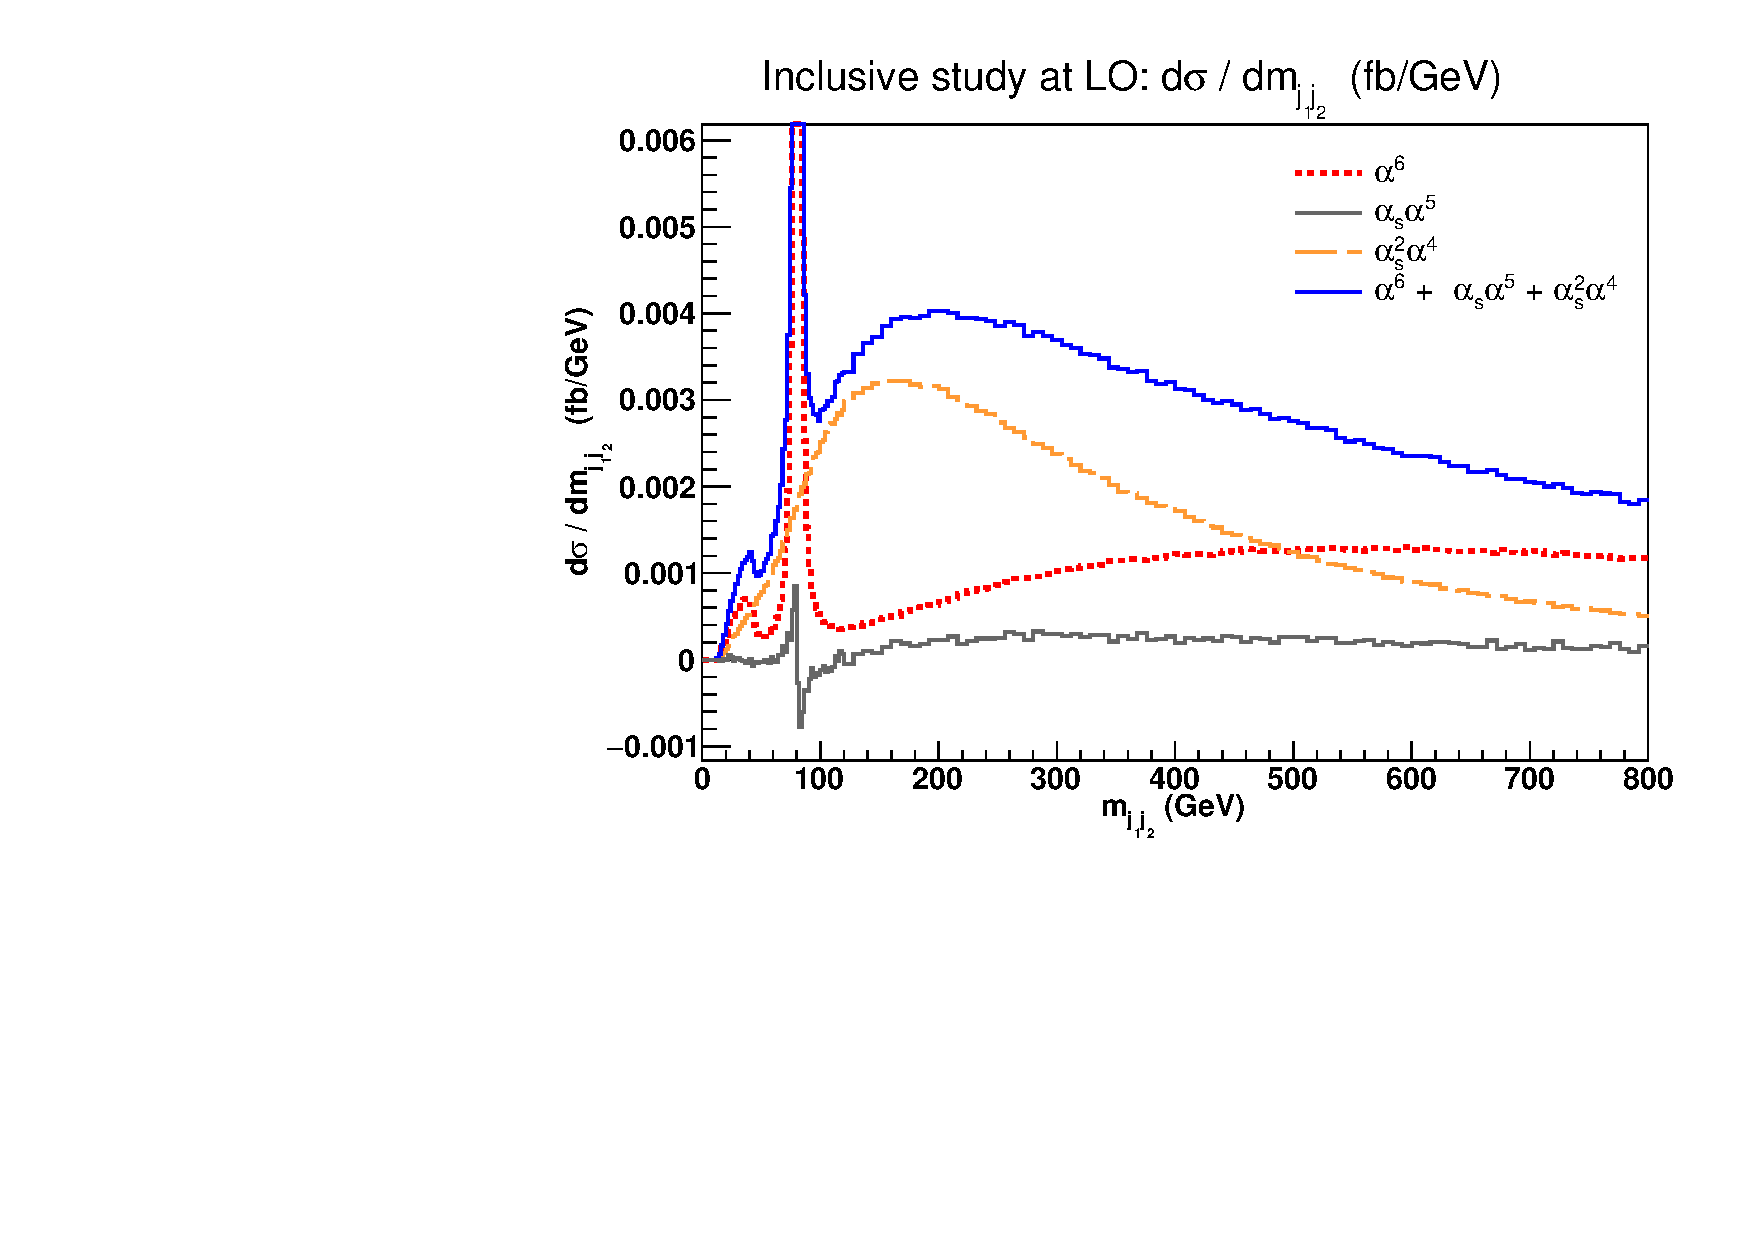
\includegraphics[scale=0.395]{../analyses/forthedraft/mjj_full.pdf}
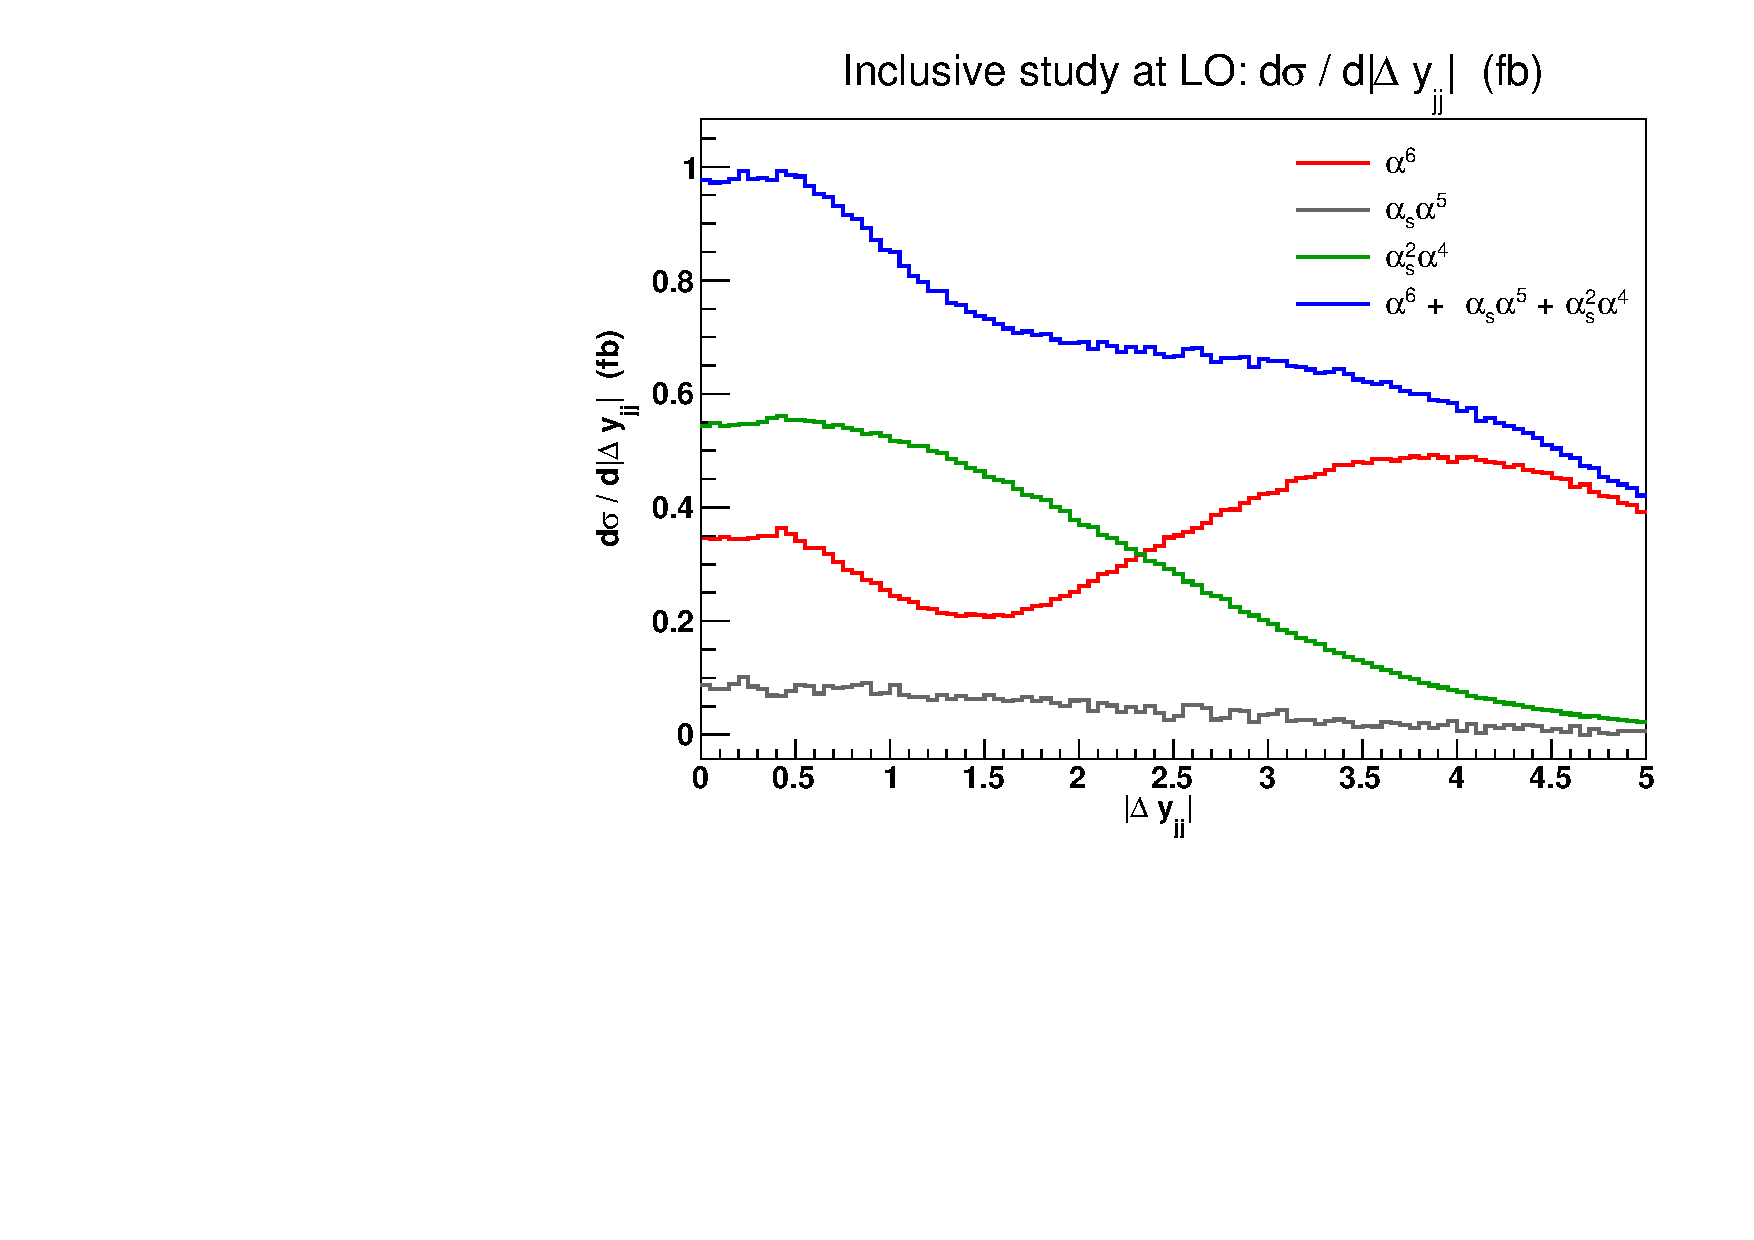
\includegraphics[scale=0.395]{../analyses/forthedraft/dyjj_full.pdf}
\caption{Differential cross--sections (fb) in $M_{jj}$ (left) and $\Delta y_{jj}$ (right) for the leading perturbative orders, without any cut on the $jj$ pair kinematics. Results of full matrix element \texttt{PHANTOM} calculations.} \label{fig:mjjdyjj_1d}
\end{figure}
\begin{figure}[ht]
\centering
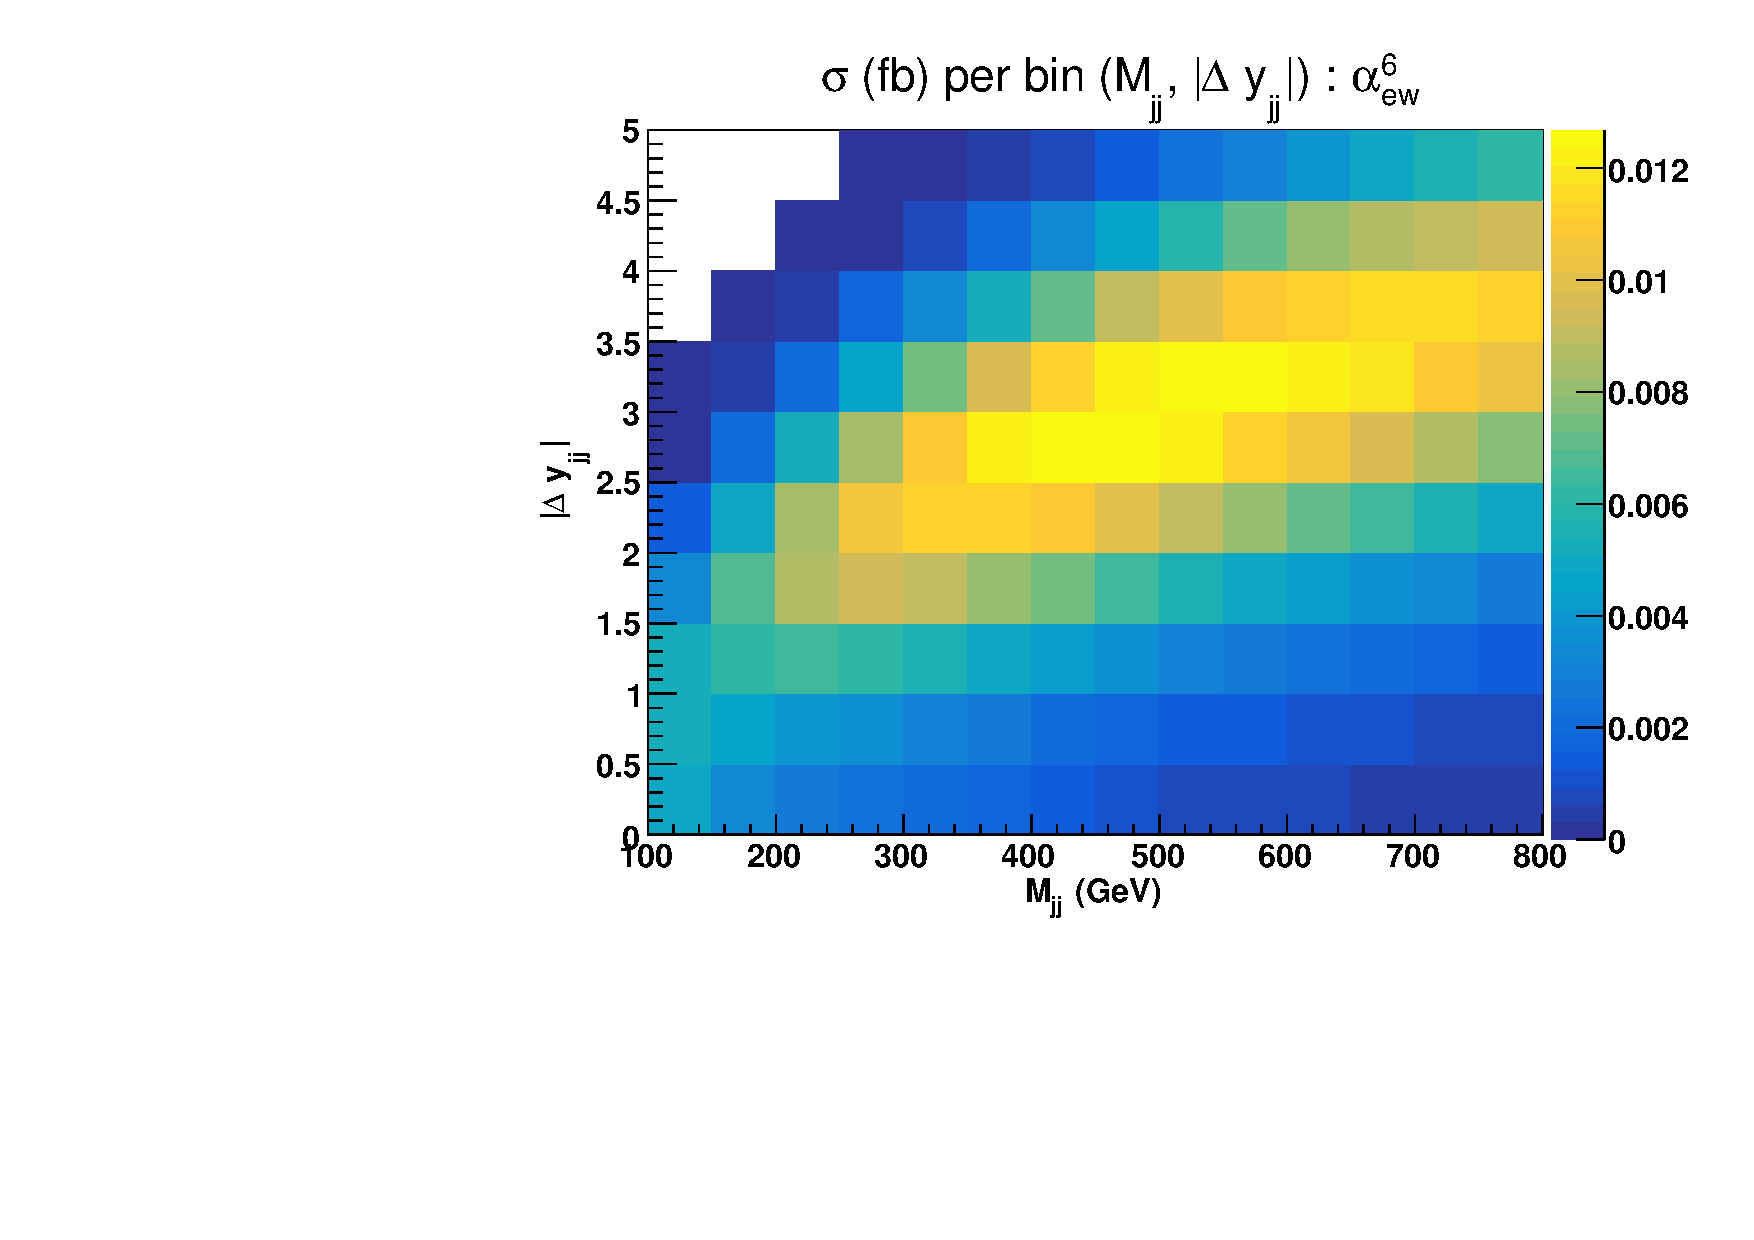
\includegraphics[scale=0.395]{../analyses/forthedraft/scan_ew6.pdf}
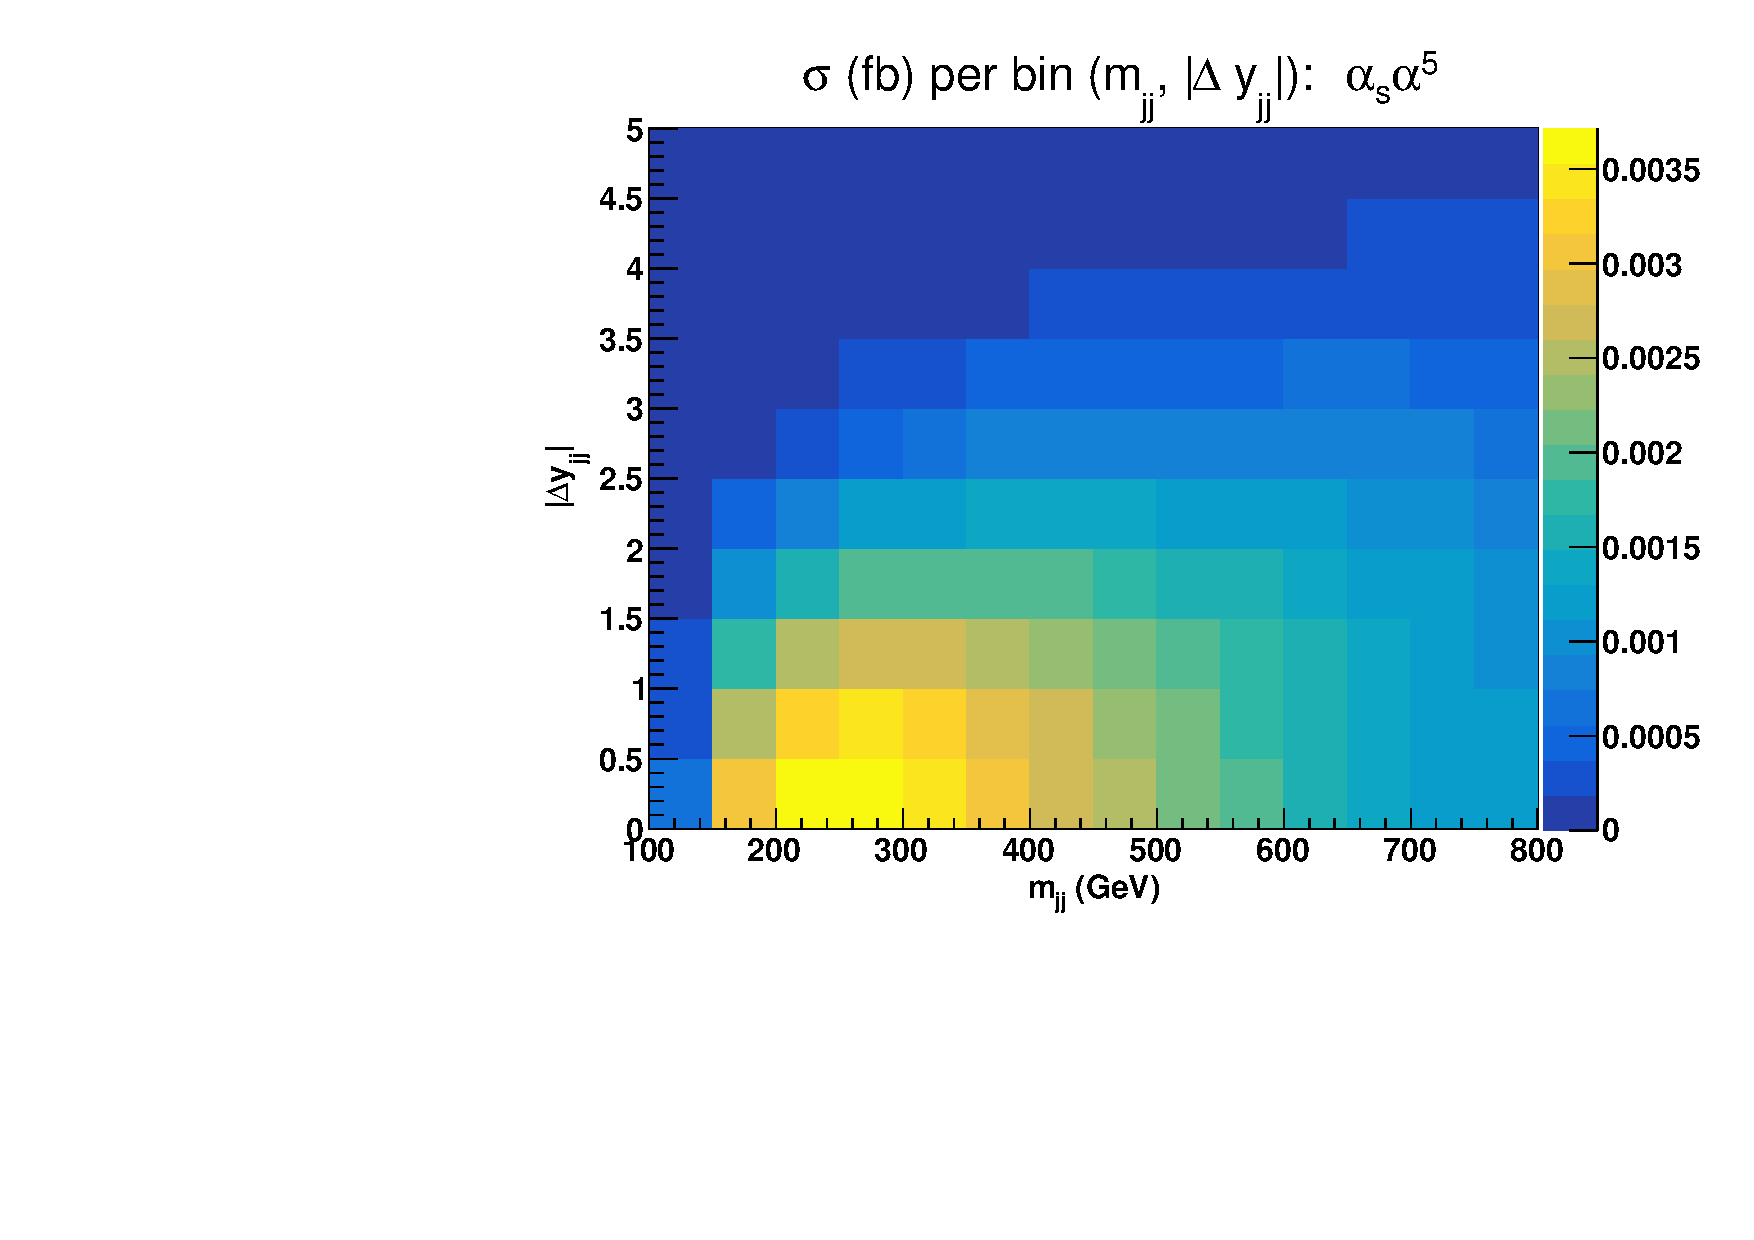
\includegraphics[scale=0.395]{../analyses/forthedraft/scan_ew5qcd1.pdf}
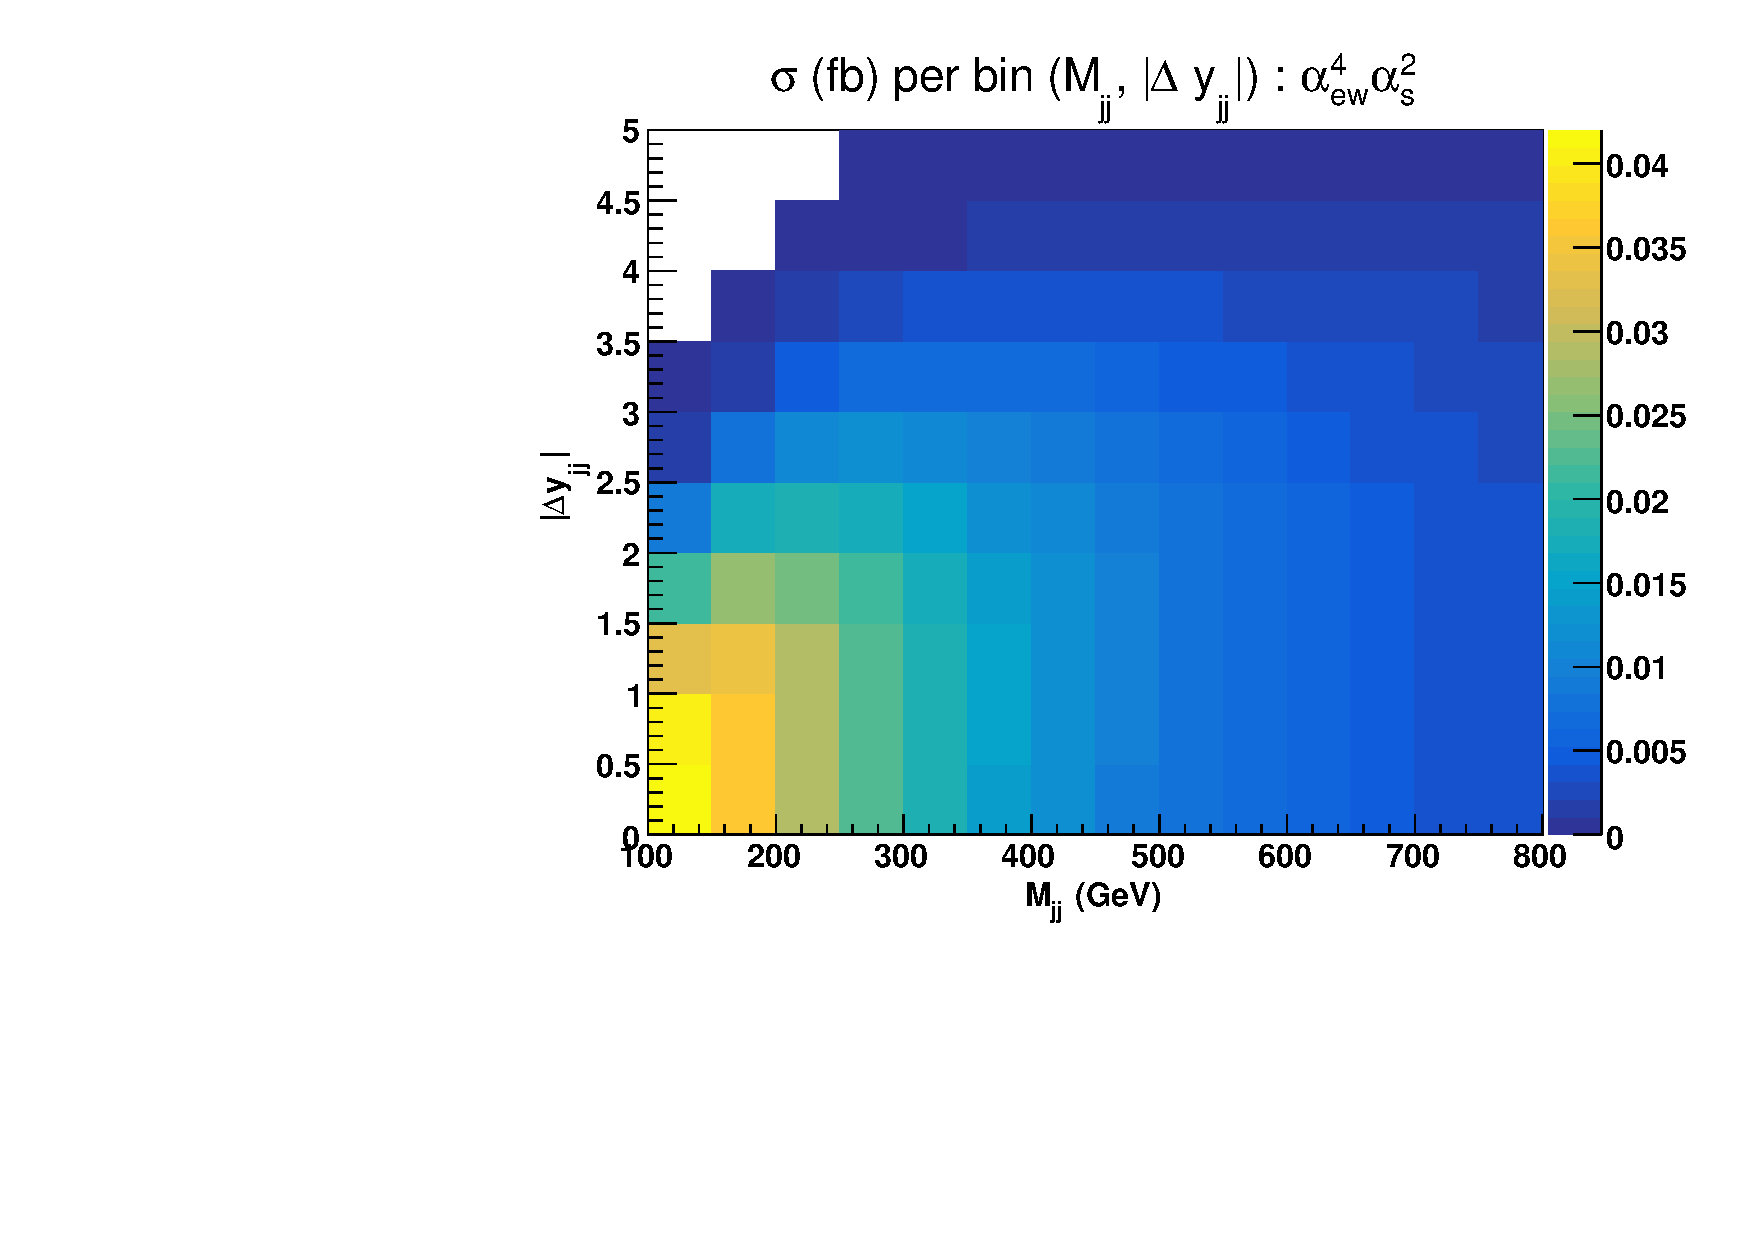
\includegraphics[scale=0.395]{../analyses/forthedraft/scan_ew4qcd2.pdf}
\caption{Cross--sections (fb) per bin of $(M_{jj},\,\Delta y_{jj})$ at the three leading perturbative orders $\mathcal{O}(\alpha_{ew}^6)$, $\mathcal{O}(\alpha_{ew}^5\alpha_s)$ and $\mathcal{O}(\alpha_{ew}^4 \alpha_s^2)$, without any cut on the $jj$ pair kinematics. Results of full matrix element \texttt{RECOLA} calculations.}\label{fig:mjjdyjj_2d_LO}
\end{figure}

\begin{figure}[hbt]
\centering
%\includegraphics[scale=0.39]{blank.pdf}
FIGURE
\caption{Cross--section (fb) per bin of $(M_{jj},\,\Delta y_{jj})$ at NLO QCD $\mathcal{O}(\alpha_{ew}^6\alpha_s)$, without any cut on the $jj$ pair kinematics. Results of \texttt{XXX} calculations.}\label{fig:mjjdyjj_2d_NLO}
\end{figure}
\newpage
\subsection{Validity of the VBS approximation}\label{subsec:VBSapprox}
\begin{figure}[hbt]
\centering
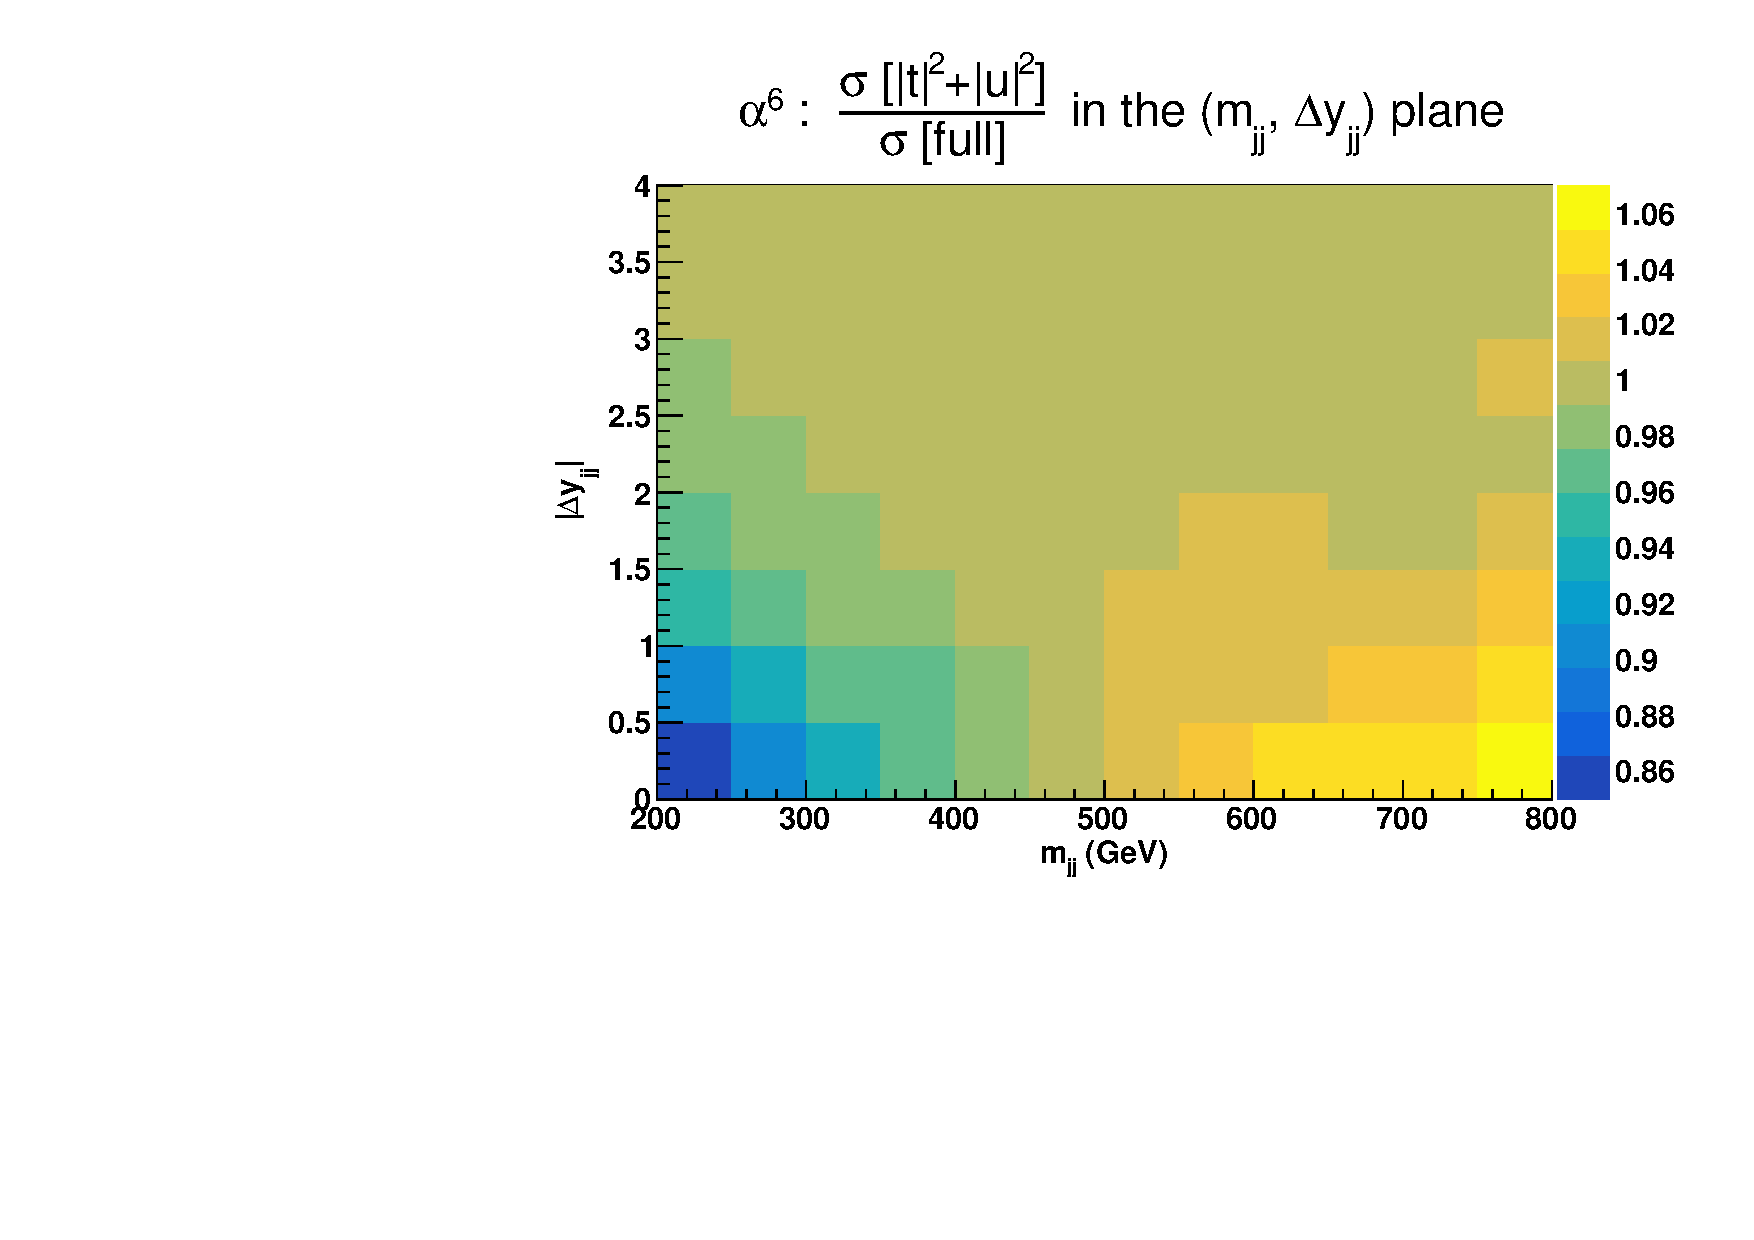
\includegraphics[scale=0.395]{../analyses/forthedraft/ratio_tu.pdf}
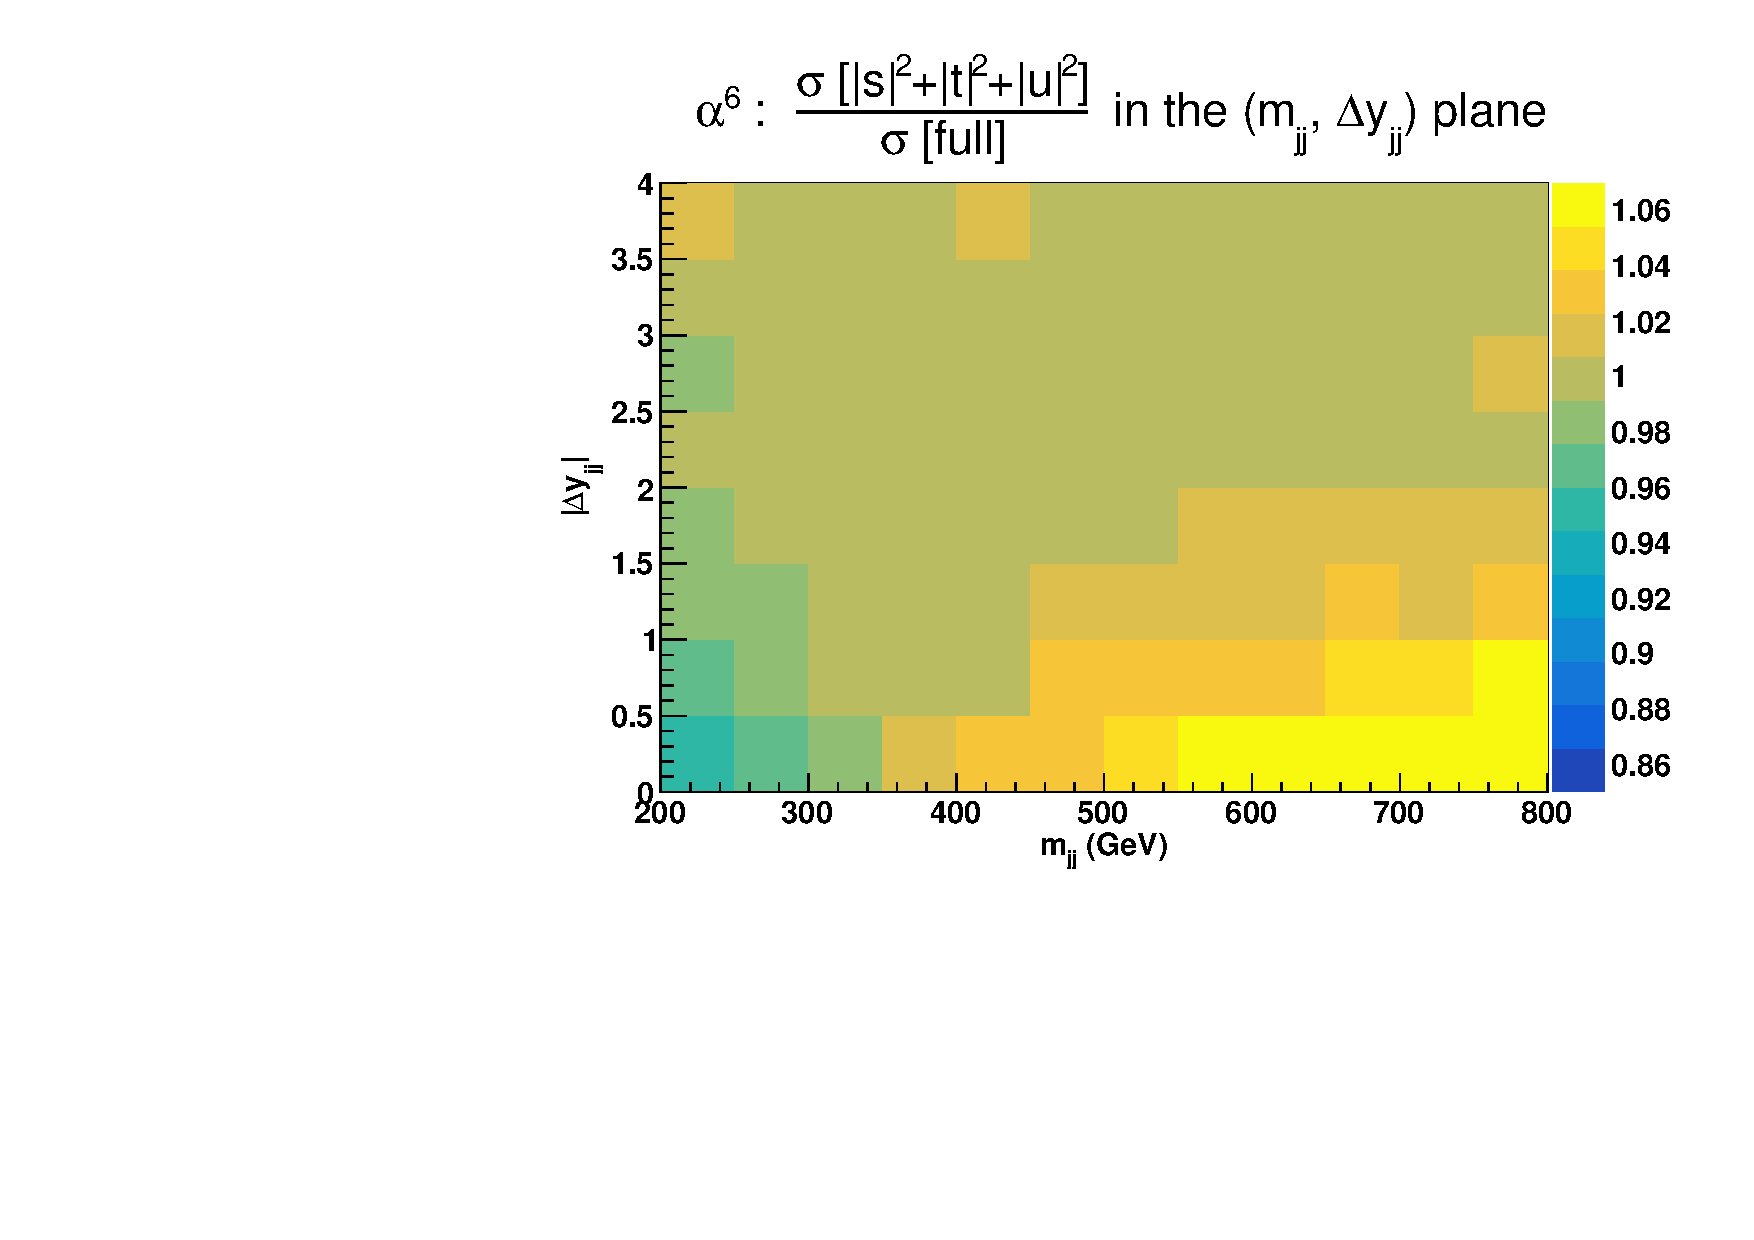
\includegraphics[scale=0.395]{../analyses/forthedraft/ratio_stu.pdf}
\caption{Cross--sections (fb) per bin of $(M_{jj},\,\Delta y_{jj})$ at $\mathcal{O}(\alpha_{ew}^6)$, without any cut on the $jj$ pair kinematics: ratio of approximated squared amplitudes over the full matrix element. The approximated squared amplitudes are computed as $|\mathcal{A}|^2 \sim |t|^2 + |u|^2$ (left) and $|\mathcal{A}|^2 \sim |s|^2 + |t|^2 + |u|^2$ (right). Results of \texttt{VBFNLO} (approximated) and \texttt{PHANTOM} (full) calculations.}\label{fig:ratio2d_LO}
\end{figure}

\begin{figure}[hbt]
\centering
%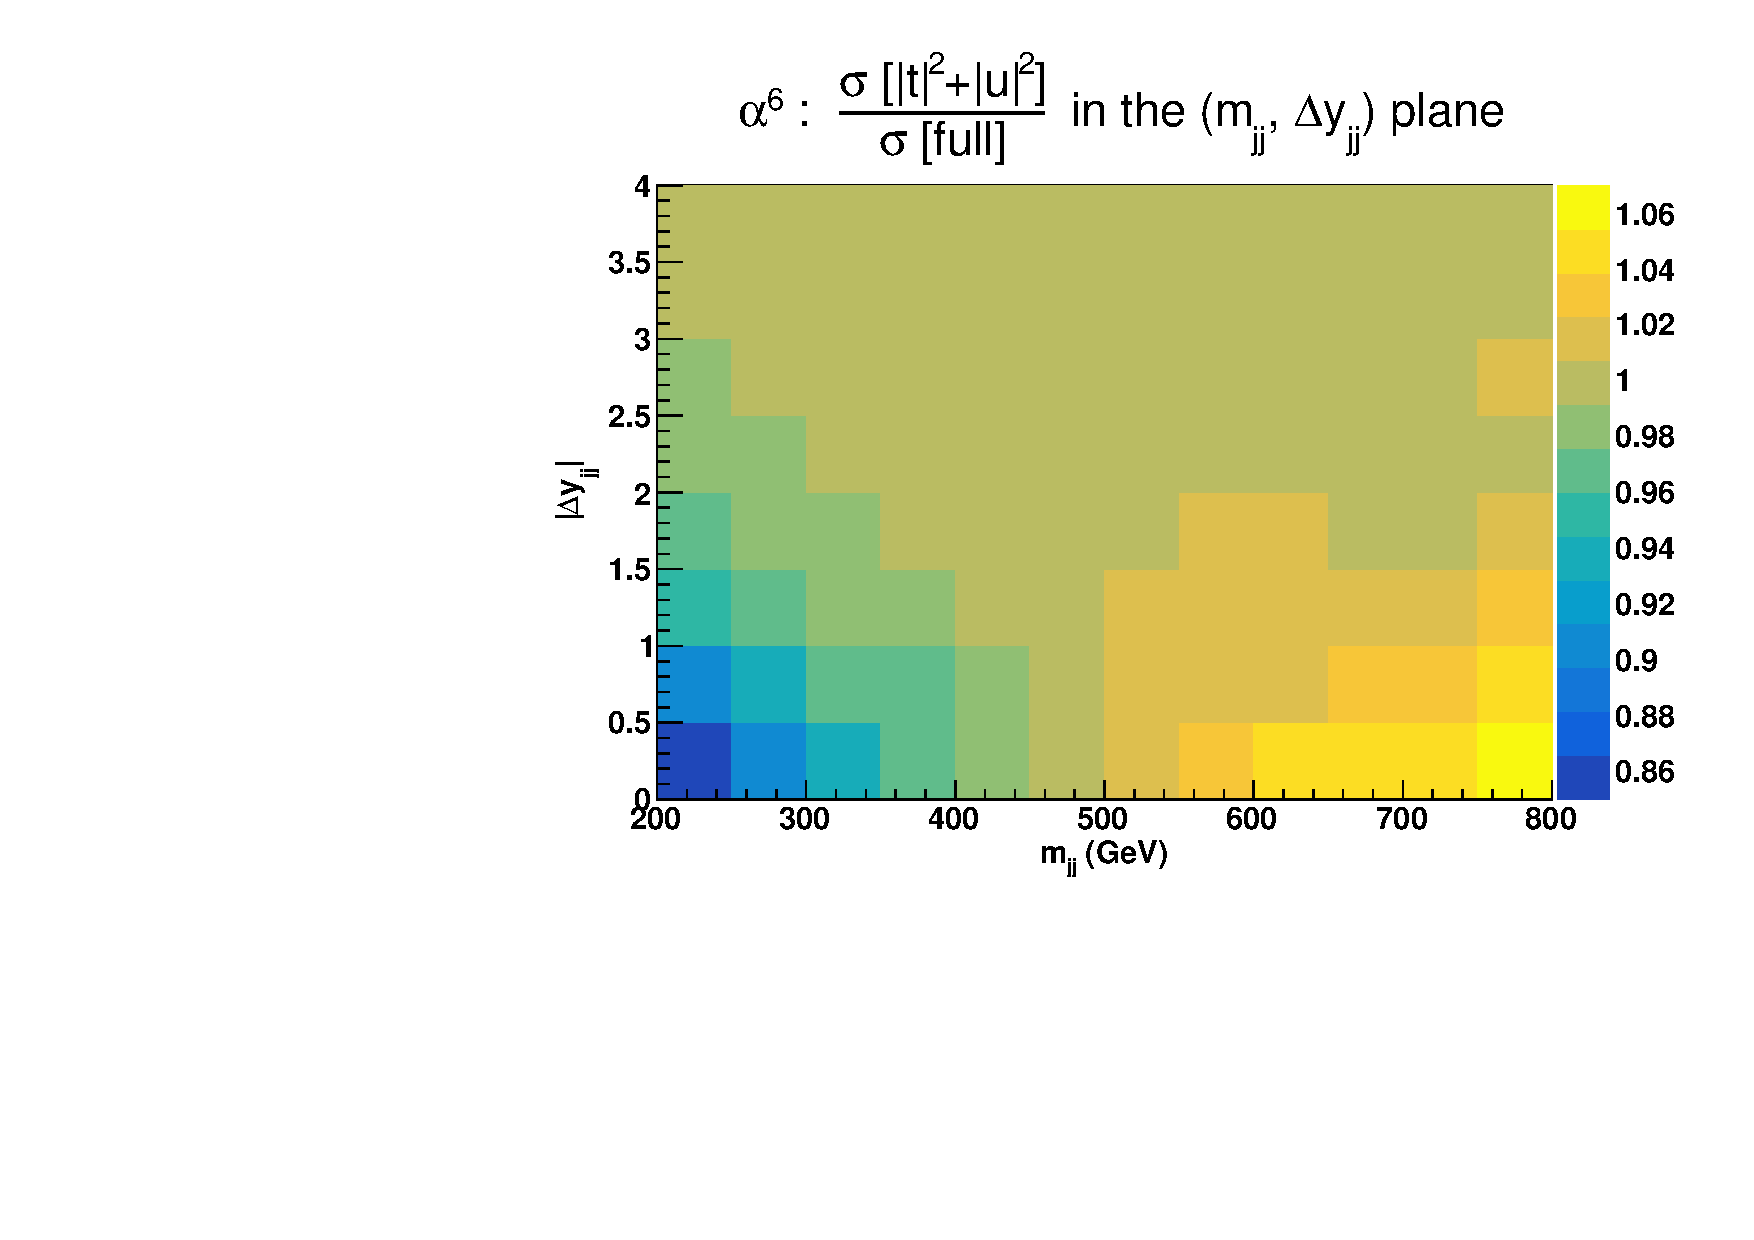
\includegraphics[scale=0.395]{../analyses/forthedraft/ratio_tu.pdf}
%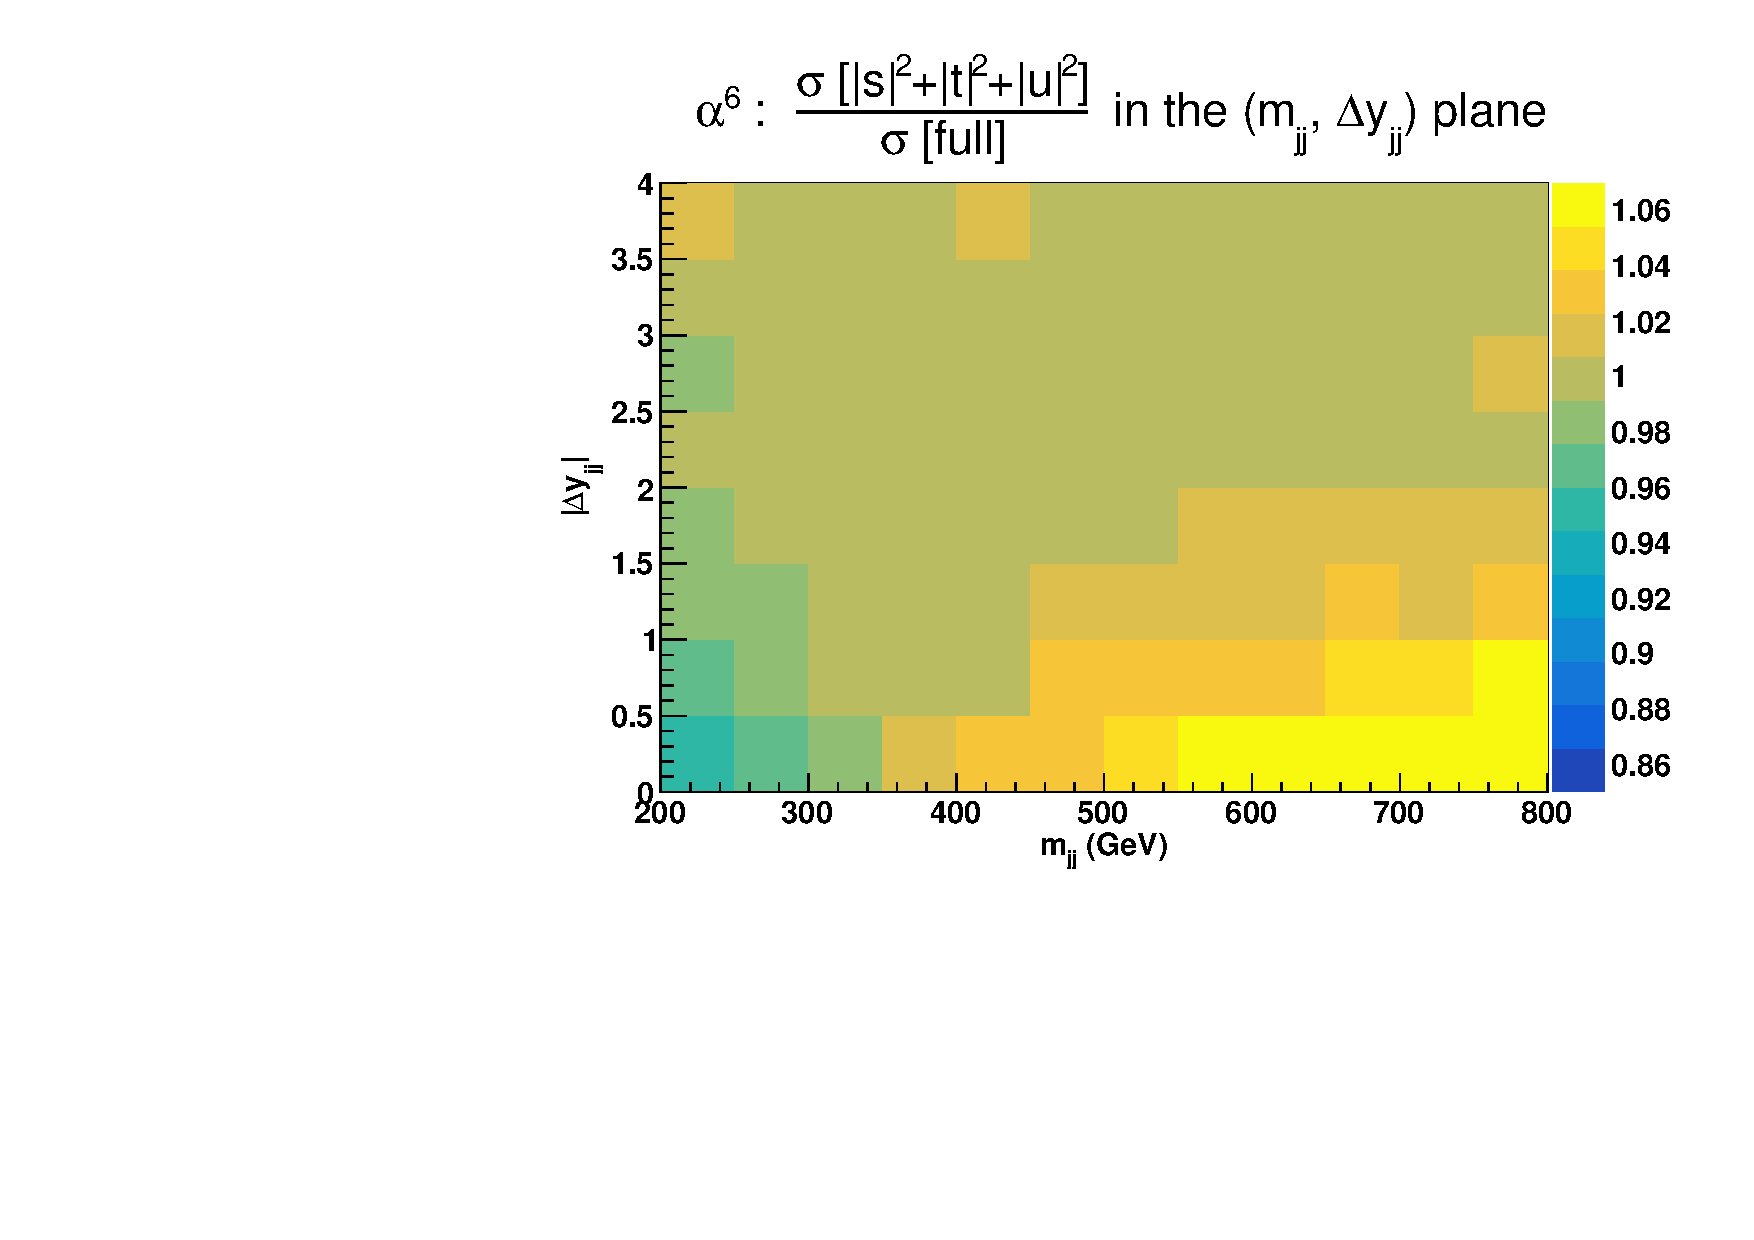
\includegraphics[scale=0.395]{../analyses/forthedraft/ratio_stu.pdf}
FIGURE
\caption{Cross--sections (fb) per bin of $(M_{jj},\,\Delta y_{jj})$ at $\mathcal{O}(\alpha_{ew}^6\alpha_s)$, without any cut on the $jj$ pair kinematics: ratio of approximated squared amplitudes over the full matrix element. The approximated squared amplitudes are computed as $|\mathcal{A}|^2 \sim |t|^2 + |u|^2$ (left) and $|\mathcal{A}|^2 \sim |s|^2 + |t|^2 + |u|^2$ (right). Results of \texttt{VBFNLO} (approximated) and \texttt{XXX} (full) calculations.}\label{fig:ratio2d_NLO}
\end{figure}